\documentclass[../main]{subfiles}

\begin{document}

\letDaniel

\noindent This week the frame of the incubator area had been built and the
circuit diagram for the 32 bit multiplexer had been drawn.

\subsection{Frame for Incubator Area}

These includes front panel, back panel, front side panels, back side panel and
back side hatch. See figure \ref{fig:partsOfIncArea} for the different assembled parts.
Figure \ref{fig:partsOfIncAreaCAD} depicts all the parts that are currently built.

\begin{figure}
    \centering
    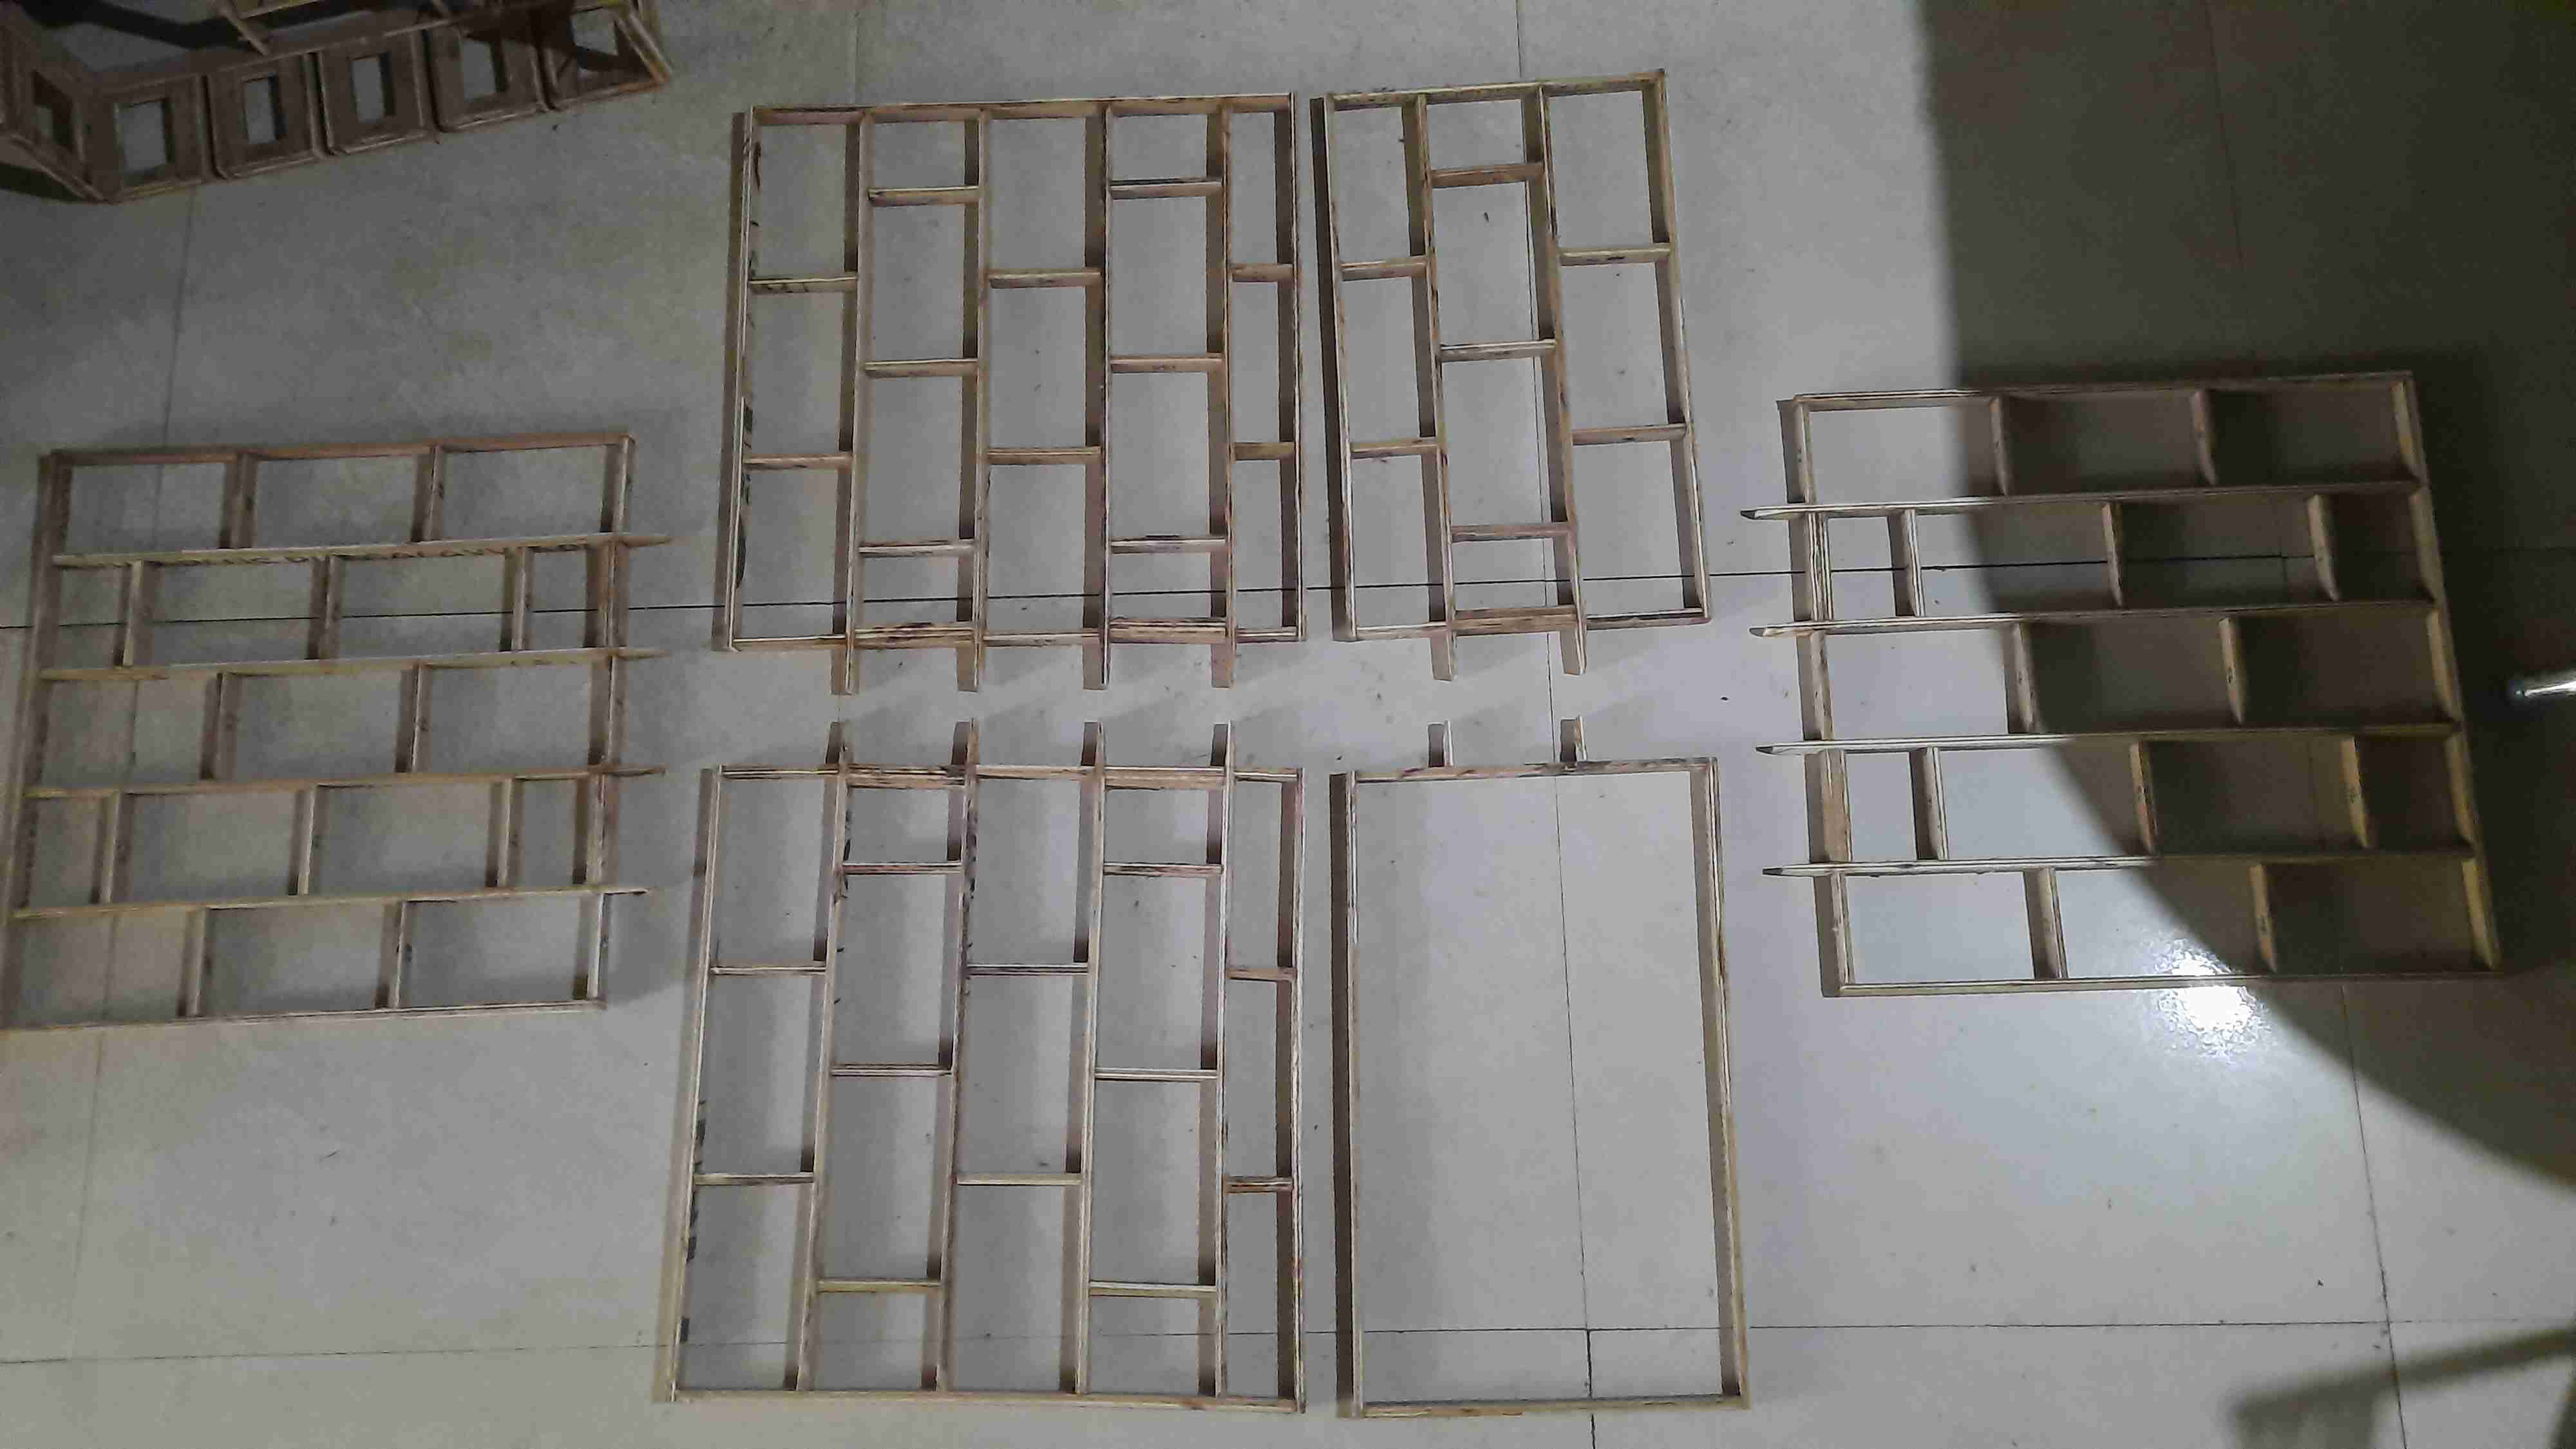
\includegraphics [
        width = 0.8\textwidth,
    ] {pics/frame_built.jpg}
    \captionof{figure} {Different assembled parts of incubator area.}
    \label{fig:partsOfIncArea}
\end{figure}

\begin{figure}
    \centering
    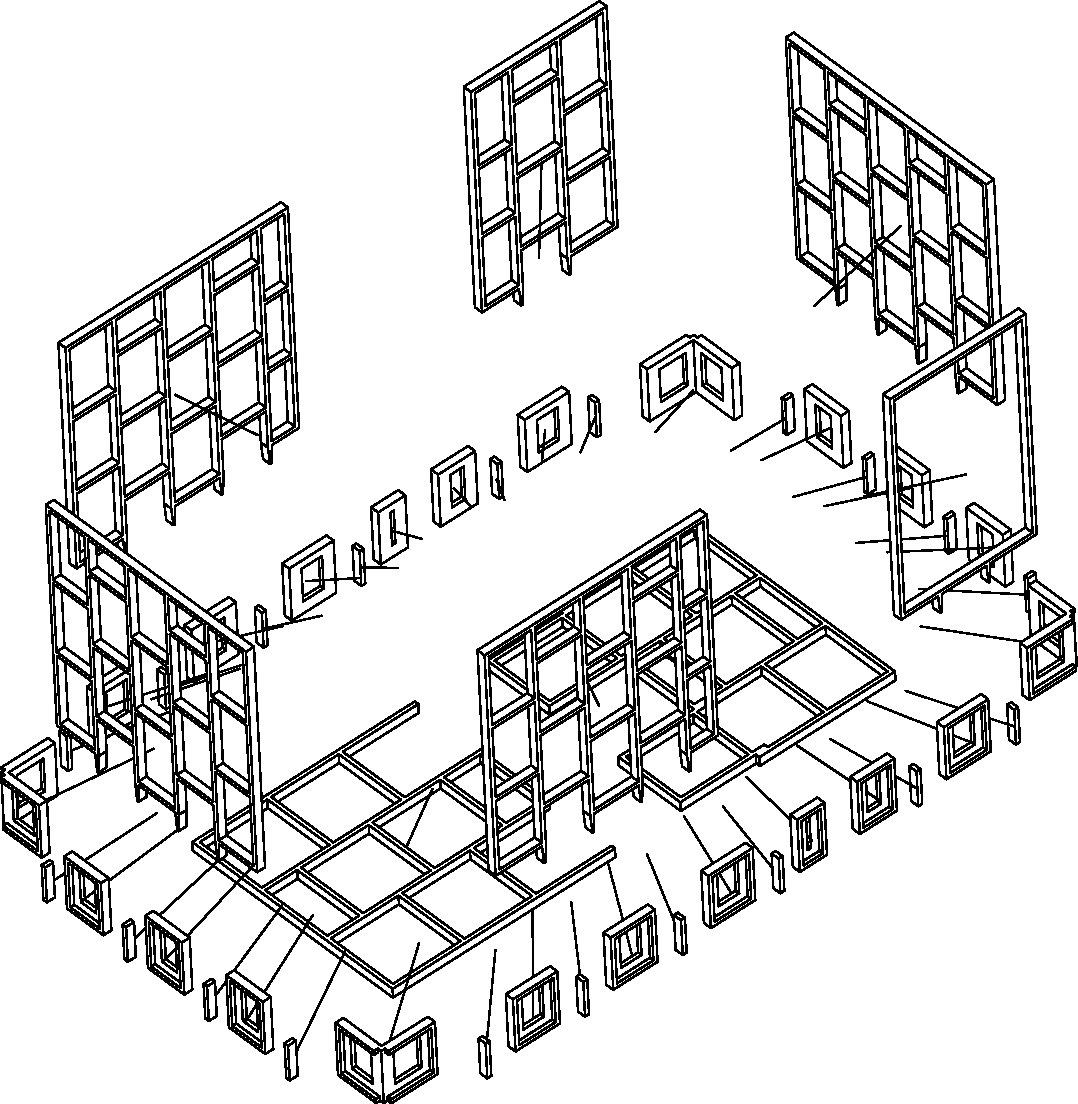
\includegraphics [
        width = 0.6\textwidth,
    ] {pics/frame_explode.pdf}
    \captionof{figure} {CAD rendering of different parts of incubator area that are completed.}
    \label{fig:partsOfIncAreaCAD}
\end{figure}

\subsection{Circuit Diagram of 32 Bit Multiplexer}

The proper circuit diagram for the 32-bit multiplexer, which had been pending
since the mini-project, was drawn this week. See figure \ref{fig:32BitMux} for
the completed circuit diagram.

\begin{figure}
    \centering
    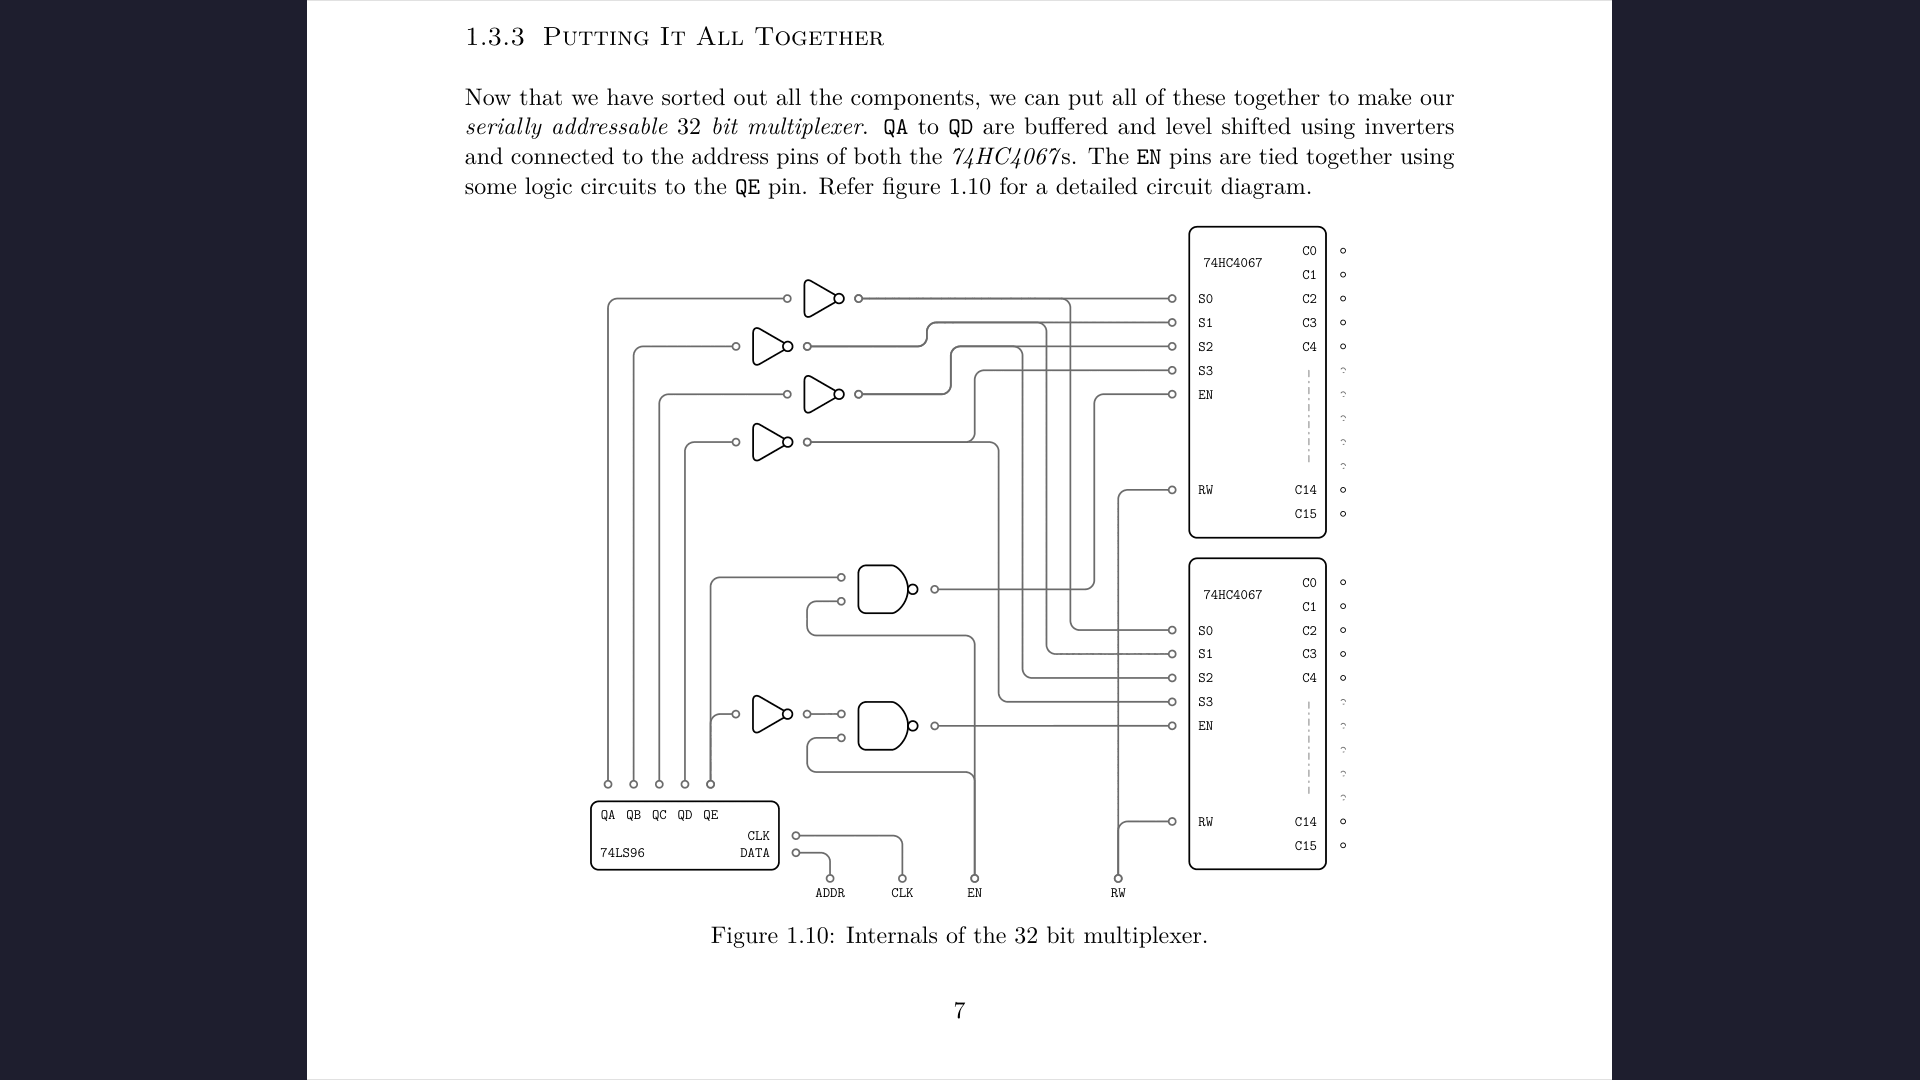
\includegraphics [
        width = 0.8\textwidth,
    ] {pics/ss1.png}
    \captionof{figure} {Screenshot showing part of the report with the multiplexer circuit.}
    \label{fig:32BitMux}
\end{figure}

% A proper circuit diagram for the 32 bit multiplexer developed as part of miniproject wasn't done yet.
% That had been taken care of in this week.

\end{document}
